\documentclass[10pt, hyperref={unicode}]{beamer}

\usepackage[czech]{babel}
\usepackage[utf8]{inputenc}
\usepackage[T1]{fontenc}
\usepackage{times} % font
\usepackage{listings} % algoritmy
\usepackage{graphics} % vkládání obrázků
\usepackage{booktabs} % kvůli toprule, midrule a bottomrule

\usetheme[progressbar=frametitle]{metropolis}
\setbeamertemplate{footline}[frame number]


\lstset{
	basicstyle=\footnotesize,
	frame=single,
	keepspaces=true,
	numbers=left,
	showstringspaces=false,
	showspaces=false,
	showtabs=false,
	tabsize=4,
}


\title{Typografie a~publikování\,--\,5.~projekt}
\subtitle{Projekt z~predmetu Databázové systémy}
\author{Matúš Fignár \,--\,xfignam00}
\date{\today}
\institute
{
	Vysoké učení technické v~Brně\\
	Fakulta informačních technologií
}

\begin{document}


\maketitle



\begin{frame}{Motivácia a cieľ projektu}
	\begin{itemize}
		\item \textbf{Cieľ}: Navrhnúť a~implementovať relačnú databázu podľa zvolenej témy.
		\pause
        \item \textbf{Téma}: Evidencia vodičov, vozidiel a~dopravných priestupkov.
        \pause
        \item \textbf{Realizácia}: Dvojčlenný tím.
        \pause
        \item \textbf{Použité technológie}: Oracle Database, PL/SQL.
        \pause
        \item \textbf{Prínos}: Precvičenie PL/SQL, návrhu databáz, analytického myslenia.
	\end{itemize}
\end{frame}


\begin{frame}[plain]{ERD}
    \centering
    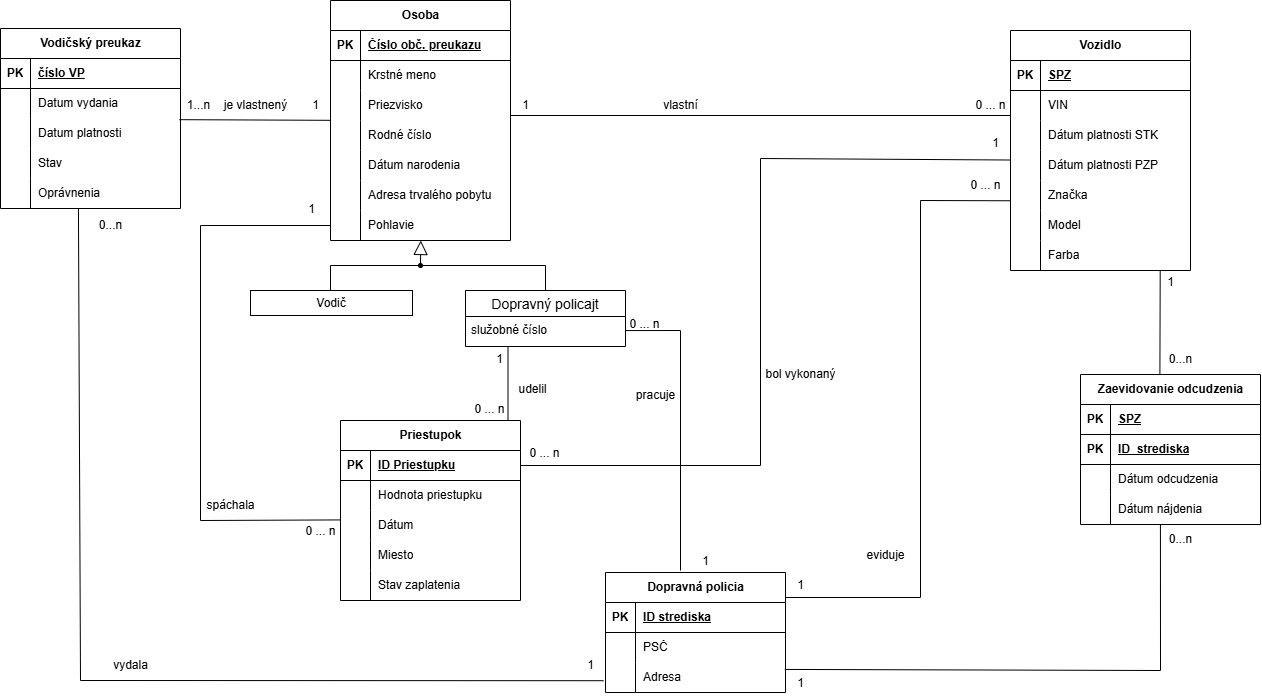
\includegraphics[width=1\textwidth]{img/ERD.png}
\end{frame}

\begin{frame}[fragile]{Tabuľky}
    \begin{itemize}
        \item Tabulky zodpovedajú ERD.
        \item Každý atribút má správne datové typy a~obmedzenia.
        \item \verb|CHECK| a~\verb|REGEXP_LIKE| na kontrolu správnosti formátu špecifických atribútov (napr. SPZ, Rodné číslo, VIN, \dots).
        \item Pri spustení databaze \texttt{DROP TABLE} na vyčistenie databázy.
    \end{itemize}
    \begin{lstlisting}[language=SQL, title={~}]
CREATE TABLE Stredisko ( 
    ID_strediska   VARCHAR(255) NOT NULL,
    PSC            VARCHAR(5) NOT NULL,
    Adresa         VARCHAR(255) NOT NULL,
    PRIMARY KEY (ID_strediska),
    CONSTRAINT PSC CHECK(REGEXP_LIKE(PSC, '^[0-9]{5}$'))
);
    \end{lstlisting}
\end{frame}


\begin{frame}[fragile]{Selecty}
    \begin{itemize}
        \item Slúžia na výpis dát z~databázy na základe špecifických dotazov.
        \item Bolo naimplementovaných 7 selektov:
        \begin{itemize}
            \item 2× JOIN
            \item 2× GROUP BY
            \item 1× EXISTS
            \item 1× IN
            \item 1× CASE -> súčasť 4. odovzdania
        \end{itemize}
    \end{itemize}
    \begin{lstlisting}[language=SQL, title={~}]
-- Vypise kolko policajtov je v jednotlivych strediskach
SELECT s.ID_strediska, 
COUNT(p.Cislo_policajta) AS Pocet_policajtov
FROM Stredisko s
LEFT JOIN Policajt p ON s.ID_strediska = p.Stredisko
GROUP BY s.ID_strediska
ORDER BY s.ID_strediska;
    \end{lstlisting}
\end{frame}


\begin{frame}[fragile]{Triggery}
    \begin{itemize}
        \item Automaticky upravujú dáta pri \texttt{INSERT}/\texttt{UPDATE}.
        \item Navrhnuté primárne na zautomatizovanie vytvárania nových položiek.
    \end{itemize}
    \begin{lstlisting}[language=SQL, title={~}]
-- Nastaveniu stavu zaplatenia na Ano ak je hodnota priestupku 0
CREATE OR REPLACE TRIGGER nastavenie_na_ano
    BEFORE INSERT OR UPDATE ON Priestupok
    FOR EACH ROW
    BEGIN
        IF :NEW.Hodnota = 0 THEN
            :NEW.Zaplatene := 'Ano';
        END IF;
    END;
    /
    \end{lstlisting}
\end{frame}


\begin{frame}[fragile]{Procedúry}
    \begin{itemize}
        \item Umožňujú opakovane vykonať komplexné operácie.
        \item Použité PL/SQL prvky: \texttt{CURSOR}, \texttt{EXCEPTION}, \verb|%ROWTYPE|.
    \end{itemize}
    \begin{lstlisting}[language=SQL, title={~}]
-- Najdenie vlastnika daneho vozidla
CREATE OR REPLACE 
    PROCEDURE najdi_vlastnika_spz(p_spz IN Vozidlo.SPZ%TYPE) IS
    vl Osoba%ROWTYPE;
BEGIN
    SELECT o.* INTO vl
    FROM Vozidlo v JOIN Osoba o ON v.Vlastnik = o.Cislo_OP
    WHERE v.SPZ = p_spz;

    DBMS_OUTPUT.PUT_LINE('Vlastnik: ' || vl.Cislo_OP);
EXCEPTION
    WHEN NO_DATA_FOUND THEN
        DBMS_OUTPUT.PUT_LINE('Vozidlo nebolo najdene');
END;
/
    \end{lstlisting}
\end{frame}

\begin{frame}[fragile]{Materializovaný pohľad}
    \begin{itemize}
        \item Statický pohľad na dáta, neuaktualizuje sa automaticky.
        \item Vytvorený medzi dvoma používateľmi s~udelenými právami.
        \item Demonštruje prístup k cudzím dátam a~výkon MV.
    \end{itemize}
    \begin{lstlisting}[language=SQL, title={~}]
-- Vypise kolko VP vydali strediska
CREATE MATERIALIZED VIEW Pocet_Vodicakov_Stredisko AS
SELECT 
    v.Vydavatel AS ID_Strediska,
    COUNT(v.Cislo_vp) AS Pocet_Vodicakov
FROM 
    xfignam00.Vodicsky_preukaz v
GROUP BY 
    v.Vydavatel;
    \end{lstlisting}
\end{frame}

\begin{frame}[fragile]{EXPLAIN PLAN}
    \begin{itemize}
        \item Zobrazenie toho ako sa planuje vykonať SQL dotaz.
        \item Použité na analýzu dotazu pred a~po vytvorení indexu.
    \end{itemize}
    \begin{lstlisting}[language=SQL, title={~}]
SELECT Pohlavie, COUNT(*) FROM Priestupok p
JOIN Osoba o ON o.Cislo_OP = p.Pokutovana_osoba GROUP BY Pohlavie;
    \end{lstlisting}
    \begin{itemize}
        \item Pred: TABLE ACCESS FULL.
        \item Po vytvorení indexu: INDEX RANGE SCAN.
        \item Výsledok: zrýchlenie dotazu
    \end{itemize}
\end{frame}


\begin{frame}[fragile]{Testovanie riešenia}
    \begin{itemize}
        \item Testovanie vykonané nad vlastnou sadou dát.
        \pause
        \item Testované: validácie, triggery, procedúry, dotazy.
        \pause
        \item Zamerané hlavne na:
        \begin{itemize}
            \item správnosť dátových obmedzení.
            \item výstupy procedúr.
            \item základnú funkcionalitu.
        \end{itemize}
        \pause
        \item Hraničné prípady testované iba čiastočne.
    \end{itemize}
\end{frame}


\begin{frame}[fragile]{Vyhodnotenie implementácie}
    \begin{itemize}
        \item Vytvorená plne funkčná a jednoduchá databáza v Oracle 12c.
        \pause
        \item Boli pokryté všetky požiadavky zadania.
        \pause
        \item Chybné časti: Pomerne triviálne triggery a procedúry.
        
    \end{itemize}
\end{frame}

\begin{frame}[c]{Záver}
    \centering
    \Huge \textbf{Ďakujem za pozornosť.}\\[1.5em]
\end{frame}

\end{document}